% Tropical character sheet by French Rice Merman

\documentclass[12pt]{article}
\usepackage{charsheet}
\usepackage{multicol}
\usepackage{amsmath}
\usetikzlibrary{fit}
%\usepackage{amsmath}
\colorlet{grayed out}{white!70!black}

\newcommand\scrm[1]{\textrm{\textsc{#1}}}

\newcommand\bigstrut{\vrule width 0pt height 16pt depth 0pt }

\usepackage{pgfkeys}

% Incomplete character support

\newcommand\fillin[1]{%
  \hbox{\vrule height 0pt depth 0.8pt width #1}%
}


\newdimen\textmargin % amount subtracted from each side to get `text width`
\textmargin=8pt

\newdimen\mynodedistance
\mynodedistance=7pt

\tikzset{%
  minimum label sep=6pt,
  every label node part/.style={
     text width=,
     font=\sffamily\footnotesize,
  },
  widecolumn/.style={
    labeled decorated stub rectangle,
    text width=134mm-2\textmargin,
    inner xsep=8pt,
    align=justify,
    font={\rightskip=0pt plus 2em},
    inner ysep=6pt,
    outer xsep=0pt, % x placement is happening by hand
    draw, line width=1.2pt,
    stub radius=2.3mm,
  },
  narrowcolumn/.style={
    widecolumn,
    text width=36mm-2\textmargin,
  },
  initiative/.style={
    labeled decorated clipped rectangle,
%    minimum width=\hpwidth/3-10pt,
    draw, line width=1.2pt,
    fill=white,
%    yseparated,
    outer xsep=3pt,
    minimum height=17mm,
  },
  dnd hit dice/.style={
    dnd max hp,
%    labeled decorated clipped rectangle,
%    yseparated,
%    minimum width=\hpwidth/2-5pt,
    minimum height=18mm,
    font=\footnotesize,
  }
}

  
\newenvironment{merman attacks}
  {\begin{minipage}{\linewidth}
   \raggedright
   \scriptsize
   \let\dndkeys=\mermanattackkeys
  }
  {\par\end{minipage}}

\makeatletter
\newcommand\mermanattackkeys[1]{%
  \gdef\@attackname{}%
  \gdef\@attackattack{}%
  \gdef\@attackdamage{}%
  \gdef\@attacktype{}%
  \gdef\@attackrange{}%
  \gdef\@attackammotype{}%
  \gdef\@attackammocount{}%
%  {\def\statdc{\protect\statdc}\typeout{attack keys: #1}}%
  \pgfkeys{/attacks/.cd, #1}%
  \hangindent=2em \hangafter=1
  \@attackname~\@attackattack, \@attackdamage~\@attacktype (\@attackrange)\par
}
\makeatother




\newcommand\fboxzero[1]{{\fboxsep=0pt \fbox{#1}}}


\begin{document}




\setDND{AGE}{400}
\setDND{ALIGNMENT}{Chaotic good}
\setDND{ARMOR CLASS}{17}
\setDND{ATTACKS}{\dndkeys{ATTACK={+11},DAMAGE={1d8+5},NAME={Black-hilt Rapier},NOTES={Magical},RANGE={5 ft.},TYPE={piercing}}
\dndkeys{AMMO COUNT={6},AMMO TYPE={daggers},ATTACK={+11},DAMAGE={1d4+5},NAME={Throwing Dagger},RANGE={20/60 ft.},TYPE={piercing}}
\dndkeys{AMMO COUNT={20},AMMO TYPE={bolts},ATTACK={+11},DAMAGE={1d6+5},NAME={Hand Crossbow},RANGE={30/120 ft.},TYPE={piercing}}}
\setDND{BACKGROUND}{Criminal}
\setDND{BONUS ACTIONS}{\bonus{Cunning Action}\relax
  \bonus{Master of Tactics}}
\setDND{CHA}{16}
\setDND{CHARACTER NAME}{Mario Greymist}
\setDND{CLASS}{Rogue}
\setDND{COLOR}{true}
\setDND{CON}{14}
\setDND{CP}{8}
\setDND{CURRENT HIT POINTS}{}
\setDND{DESCRIPTION}{A nondescript Dragaeran male who can blend into any crowd.  Has a round face like a Teckla, but also has a noble's point.  Resembles a friendly and somewhat elderly merchant.}
\setDND{DEX}{20}
\setDND{DEX SAVING}{true}
\addDNDitem{LIGHT WEAPONS}{Throwing Daggers}
\addDNDitem{NORMAL WEAPONS}{Black-hilt Rapier}
\addDNDitem{NORMAL WEAPONS}{Hand Crossbow}
\addDNDitem{LIGHT ARMOR}{Glamoured Studded Leather Armor}
\addDNDitem{LIGHT ARMOR}{Cloak of Protection}
\addDNDitem{LIGHT ARMOR}{Boots of Elvenkind}
\addDNDitem{SLOTTED ITEMS}{Crossbow Bolts}
\addDNDitem{SLOTTED ITEMS}{Potion of Invisibility}
\addDNDitem{SLOTTED ITEMS}{Fine Clothes}
\addDNDitem{SLOTTED ITEMS}{Forged Papers}
\addDNDitem{SLOTTED ITEMS}{Poison Vials (3)}
\addDNDitem{SLOTTED ITEMS}{Marked Cards}
\addDNDitem{SLOTTED ITEMS}{Thieves' Tools}
\addDNDitem{SLOTTED ITEMS}{Disguise Kit}
\addDNDitem{SLOTTED ITEMS}{Forgery Kit}
\addDNDitem{SMALL ITEMS}{Ring of Mind Shielding}
\addDNDitem{SMALL ITEMS}{Sending Stone}
\addDNDitem{SMALL ITEMS}{Blackmail Ledger}
\setDND{EQUIPMENT}{\item Throwing Daggers
\item Black-hilt Rapier
\item Hand Crossbow
\item Glamoured Studded Leather Armor
\item Cloak of Protection
\item Boots of Elvenkind
\item Crossbow Bolts
\item Potion of Invisibility
\item Fine Clothes
\item Forged Papers
\item Poison Vials (3)
\item Marked Cards
\item Thieves' Tools
\item Disguise Kit
\item Forgery Kit
\item Ring of Mind Shielding
\item Sending Stone
\item Blackmail Ledger}
\setDND{EQUIPMENT COLS}{2}
\setDNDfont{EQUIPMENT}{\scriptsize}
\setDND{EQUIPMENT LEFT}{true}
\setDND{FEATURES}{\describedColored{attacks}{Sneak Attack}{Once per turn, Mario deals an extra 10d6 damage to a creature he hits with a finesse or ranged weapon attack when he has advantage or an ally threatens the target.}
\described{Cunning Action \upshape{[B]}}{Mario may Dash, Disengage, or Hide as a bonus action.}
\described{Uncanny Dodge \upshape{[Rx]}}{When an attacker Mario can see hits him with an attack, he may halve the attack's damage.}
\described{Evasion}{When subjected to an effect allowing a Dexterity saving throw for half damage, Mario instead takes no damage on a success and only half damage on a failure.}
\described{Reliable Talent}{Any ability check using a proficient skill or tool treats rolls lower than 10 as a 10.}
\described{Blindsense}{Mario is aware of hidden or invisible creatures within 10 feet.}
\described{Slippery Mind}{Mario gains proficiency in Wisdom saving throws.}
\described{Elusive}{No attack roll has advantage against Mario while he is conscious.}
\describedColored{attacks}{Stroke of Luck}{Once per short rest, Mario may turn a missed attack into a hit or treat a failed ability check as a natural 20.}
\described{Master of Intrigue}{Mario mimics speech patterns and accents easily and excels at maintaining false identities.}
\described{Master of Tactics \upshape{[B]}}{Mario may use the Help action as a bonus action at a range of 30 feet.}
\described{Insightful Manipulator}{After observing or conversing with someone for one minute, Mario can assess whether the creature surpasses him in Intelligence, Wisdom, Charisma, or class levels.}
\describedColored{attacks}{Misdirection \upshape{[Rx]}}{When targeted by an attack while another creature is nearby, Mario may cause the attack to target the other creature instead.}
\described{Soul of Deceit}{Mario's thoughts cannot be read by telepathy unless he allows it, and he presents false thoughts when magically compelled.}}
\setDNDfont{FEATURES}{\footnotesize}
\setDND{FEATURES SPACE}{3pt}
\setDND{GP}{320}
\setDND{HIT DICE}{d8}
\setDND{INITIATIVE}{+11}
\setDND{INT}{12}
\setDND{INT SAVING}{true}
\setDND{LAYOUT}{silverpine}
\setDND{LEVEL}{20}
\setDND{MAX HP}{143}
\setDND{MOTIVATION}{Avenge insults to his beloved.}
\setDND{PASSIVE INSIGHT}{18}
\setDND{PASSIVE PERCEPTION}{18}
\setDND{PLAYER NAME}{Steve}
\setDND{PP}{12}
\setDND{PROFICIENCIES}{\item Perception
\item Sleight of Hand
\item Acrobatics
\item Deception
\item Insight
\item Investigation
\item Persuasion
\item Stealth
\profskip{}
\item Thieves' Tools
\item Disguise Kit
\item Forgery Kit
\item Poisoner's Kit
\profskip{}
\item Daggers
\item Hand Crossbows
\item Longswords
\item Rapiers
\item Shortswords
\profskip{}
\item Common
\item Dragaeran
\item Eastern
\item Thieves' Cant}
\setDND{PROFICIENCY BONUS}{+6}
\setDND{RACE}{Dragaeran}
\setDND{REACTIONS}{\reaction{Uncanny Dodge}\relax
  \reaction{Misdirection}}
\setDND{SENSES}{Darkvision 60 ft.}
\setDND{SHEET ORIGIN}{Mario Greymist (Jhereg assassin)}
\setDND{SP}{15}
\setDND{SPECIALTY}{Assassin}
\setDND{SPEED}{30}
\setDND{STR}{10}
\setDND{WIS}{15}

\DNDinit

\noindent
\begin{charsheet}[x=1mm,y=1mm,inner sep=0pt]
  \tikzset{node distance=\mynodedistance}

\node [anchor=south west] (merman) at (0,0) {
   \vbox{
    \vspace*{15mm}
   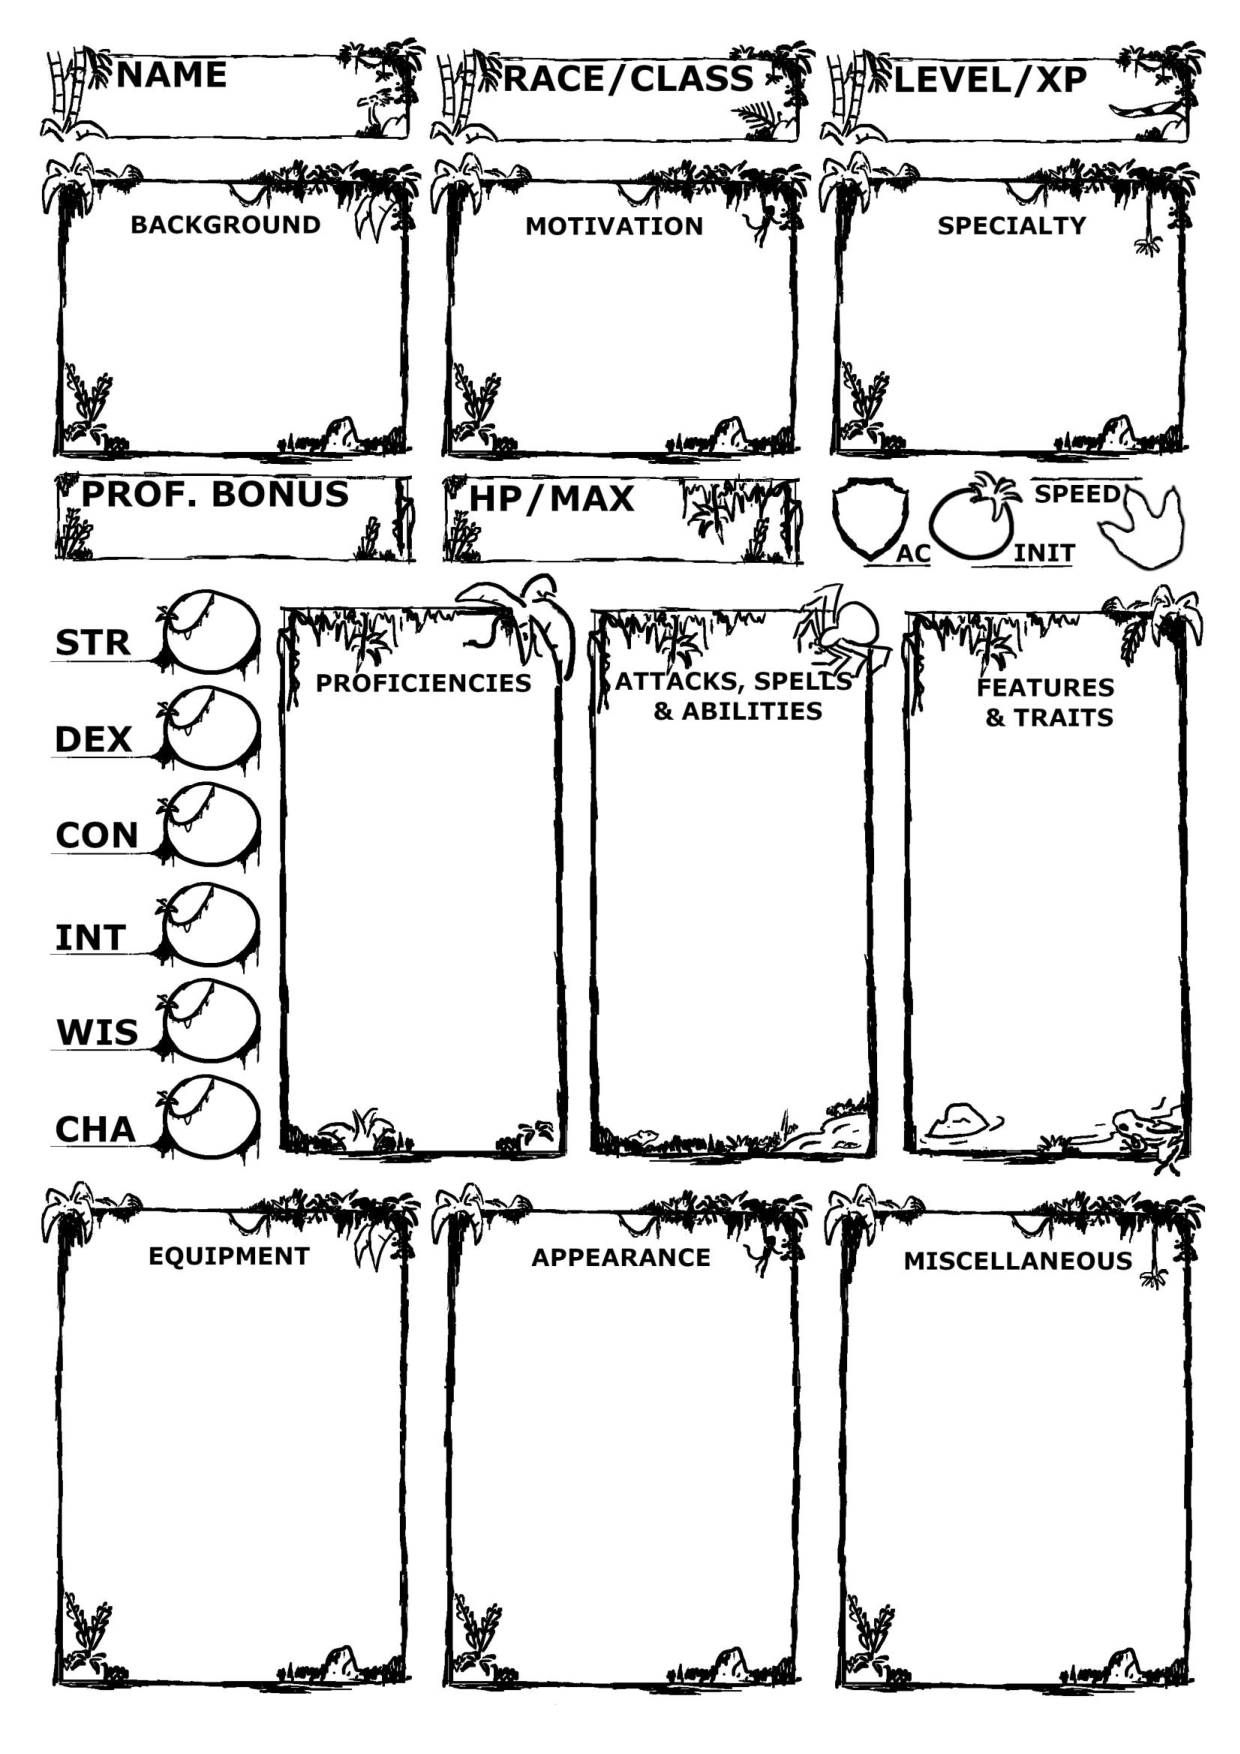
\includegraphics[height=\paperheight]{templates/merman.pdf}
    \vspace*{-15mm}
   }
};

\path [opacity=0.57,fill=white] (merman.south west) rectangle (merman.north east);

% Grid overlay: thin line every 1mm, heavy every 10mm, labels every 10mm.
% Grid is anchored to the image's SW corner so labels align with gridlines.
% NB: charsheet env uses x=1cm,y=1cm, so step must be given with explicit mm
% units (otherwise step=1 means 1cm and the thin grid coincides with the heavy).

\iffalse

    \begin{scope}
      \clip (merman.south west) rectangle (merman.north east);
      \draw[blue!40, line width=0.1pt]
        (merman.south west) grid[step=1mm] (merman.north east);
      \draw[blue!60, line width=0.8pt]
        (merman.south west) grid[step=10mm] (merman.north east);
      \foreach \x in {0,10,...,300} {
        \node[anchor=south west, font=\tiny\sffamily\bfseries,
              text=blue, inner sep=1pt]
          at ([xshift=\x mm]merman.south west) {\x};
      }
      \foreach \x in {0,10,...,300} {
        \path ([xshift=\x mm]merman.south west) ++(0,180mm) 
           node [anchor=north west, font=\tiny\sffamily\bfseries,
                 text=blue, inner sep=1pt]
           {\x}
           ;
      }
      \foreach \y in {10,20,...,300} {
        \node[anchor=south west, font=\tiny\sffamily\bfseries,
              text=blue, inner sep=1pt]
          at ([yshift=\y mm]merman.south west) {\y};
      }
    \end{scope}

\fi


\LARGE
\sffamily
\bfseries
\color{blue!60!black}

\path (41,169.5) node (STR)  {\dndmodifier{STR}}
    ++(0, -15.5)  node (DEX) {\dndmodifier{DEX}}
    ++(0, -15.5)  node (CON) {\dndmodifier{CON}}
    ++(0, -15.7)  node (INT) {\dndmodifier{INT}}
    ++(0, -15.5)  node (WIS) {\dndmodifier{WIS}}
    ++(0, -15.5)  node (CHA) {\dndmodifier{CHA}}
;


\begin{scope}
\large
\tikzset{anchor=north}

\path (21,163) node (STR)  {\getDND*{STR}}
    ++(0, -15.5)  node (DEX) {\getDND*{DEX}}
    ++(0, -15.5)  node (CON) {\getDND*{CON}}
    ++(0, -15.7)  node (INT) {\getDND*{INT}}
    ++(0, -15.5)  node (WIS) {\getDND*{WIS}}
    ++(0, -15.5)  node (CHA) {\getDND*{CHA}}
;

\end{scope}

\normalsize

\path (168,0) coordinate (right center);
\path (44,0) coordinate (left center);
\path (105,0) coordinate (center);

\path(0,250) coordinate (top baseline);

\begin{scope}
\tikzset{anchor=south}
\node [anchor=south] (race/class) at (top baseline -| left center) {\getDND*{CHARACTER NAME}};

\node [anchor=south] (race/class) at (top baseline -| center) {\getDND*{RACE}/\getDND*{CLASS}};

\node [anchor=south] (level/xp) at (top baseline -| right center)
         {\getDND*{LEVEL} / \fillin{1in}}
  ;

\path (0,183) coordinate (hp baseline);

 \node [anchor=south] (proficiency bonus) at (left center |- hp baseline)
       {+\arabic{proficiency bonus}}
    ;

\node [anchor=south] (hp/max) at (center |- hp baseline)
 {\fillin{2cm} / \getDND*{MAX HP}\hspace*{1cm}};

\path (hp baseline) ++(0,2) coordinate (ac baseline);

\path (144.5,0 |- ac baseline) ++(0,1) node {\large\getDND*{ARMOR CLASS}};

\path (161.0,0 |- ac baseline) ++(0,-0.5) node {\whenDNDdefined{INITIATIVE}{\signed{\rawgetDND{INITIATIVE}}}};

\path (189.7,0 |- hp baseline) ++(0,-1) node {\getDND*{SPEED}};

\tikzset{anchor=north}

\path (0, 230) coordinate (bg top);

\node [anchor=north] (background) at (bg top -| left center) {\getDND*{BACKGROUND}};

\node (motivation) at (bg top -| center)
      {\begin{minipage}{4cm}\centering\getDND*{MOTIVATION}\end{minipage}};

\node (specialty) at (bg top -| right center)
      {\begin{minipage}{4cm}\centering\getDND*{SPECIALTY}\end{minipage}};


\end{scope}

 \node (proficiencies)
     [text width=4.2cm,
      anchor=north,
     ]
   at (72, 160)
  { \useDNDfont*{PROFICIENCIES}
    \newif\ifprofs
    \scriptsize
    \profsfalse
    \whenDNDnonempty{PROFICIENCIES}\profstrue
%    \whenDNDnonempty{SECONDARY PROFICIENCIES}\profstrue
    \begin{proflist}
    \let\profskip=\smallskip
    \raggedright
    \getDND*{PROFICIENCIES}
%    \whenDNDnonempty{PROFICIENCIES}{%
%        \whenDNDnonempty{SECONDARY PROFICIENCIES}{\profskip}}
%    \getDND*{SECONDARY PROFICIENCIES}
    \relax
    \ifprofs\else \item (No proficiencies listed.)\fi
    \end{proflist}
  }
;



\node (attacks etc) [anchor=north, text width=4.3cm] at (124, 153)
     {
     \centering
     \useDNDfont*{ATTACKS}
     \noindent
    \let\small=\tiny
     \begin{merman attacks}
     \gdef\notesheader{\cline{2-4}}%
     \gdef\notesheader{}%
     \gdef\attacknote#1#2{}%  Just don't
     \getDND*{ATTACKS}%

     \whenDNDdefined{MAGIC}
     {
      \par\smallskip
      \advance\baselineskip by 2pt \selectfont
      \def\spellslevellabel#1#2{\ignorespaces\relax}%
      \long\def\describedColored#1#2#3{\emph{#2}\\}%
      \long\def\described#1#2{\emph{#1}\\}%
      \rawgetDND{MAGIC}%
     }
     \end{merman attacks}
  }
  ;
  

  \whenDNDdefined{FEATURES}{
      \node[text width=4.3cm, anchor=north] 
       (features)
        at (173, 0 |- attacks etc.north)
       {\long\def\described#1#2{%
           \hangindent=2em \hangafter=1
           \scriptsize #1: \tiny #2 \par
        }
        \def\describedColored#1{\described}%
        \begin{merman attacks}
        \parskip=2.5pt
        \let\rlapequip\relax
        \getDND{FEATURES}
        \end{merman attacks}
       };
  }

\path (right center) coordinate (bottom right center);
\path (42,0) coordinate (bottom left center);
\path (center) coordinate (bottom center);

\path (0, 68) coordinate (equipment top);

  \whenDNDdefined{EQUIPMENT}{%
      \node[text width=4.3cm, anchor=north] 
       (equipment)
        at (bottom left center |- equipment top)
        {
          \begin{minipage}{\linewidth}
          \scriptsize
          \begin{eqlist}%
         \ifDNDnonempty{EQUIPMENT}
            {\getDND{EQUIPMENT}}
            {\item (Placeholder: Equipment will go here.)}%
         \end{eqlist}
         \end{minipage}%
       }
      ;
  }

  \whenDNDdefined{DESCRIPTION}{%
      \node[text width=4.3cm, anchor=north] 
       (equipment)
        at (bottom center |- equipment top)
        {
          \begin{minipage}{\linewidth}
          \vspace*{0.5\baselineskip}
          \hyphenpenalty=9000
          \exhyphenpenalty=9000
          \getDND{DESCRIPTION}
          \end{minipage}%
       }
      ;
  }


%%%%      \node (equipment) [draw=none,fill=none,left of lower corner=of features] {};
%%%%    }
%%%%    
%%%%    \path (equipment.north west) +(3mm,-\mynodedistance) coordinate (coin top left);
%%%%    
%%%%    \coin{cp}{Cu}{\color{grayed out}\getDND*{CP}}
%%%%    \coin{sp}{Ag}{\color{grayed out}\getDND*{SP}}
%%%%    \coin{gp}{Au}{\color{grayed out}\getDND*{GP}}
%%%%    \coin{pp}{Pt}{\color{grayed out}\getDND*{PP}}
%%%%      
%%%%    \setdeltax\sectionwidth{attacks.west}{stats background.east}
%%%%    \path (stats background.east) ++(\mynodedistance,0) ++(-2.5pt,0) coordinate (prof circle west);
%%%%    \node (proficiency circle) [anchor=west,proficiencies,circle,
%%%%           width=10mm,height=10mm,line width=1.5pt,draw]
%%%%           at (prof circle west |- proficiency bonus.center)
%%%%          {\large\textsf{+\arabic{proficiency bonus}}};
%%%%    
%%%%    \draw [line width=0.5pt] (proficiency circle) circle [radius=4.2mm];
%%%%    
%%%%    % center the text in the visible space
%%%%    \setdeltax\tmpwidth{proficiency bonus.east}{proficiency circle.east}
%%%%    
%%%%    % proficiencies bottom should be stats background bottom or equipment
%%%%    % top, whatever is higher
%%%%    
%%%%    
%%%%      \setdeltay\tmpheight{stats background.south}{equipment.north}
%%%%      \advance\tmpheight by -\mynodedistance % allows space above equipment.north
%%%%      \ifdim\tmpheight>0pt
%%%%        \setdeltay\sectionheight{proficiency bonus.south}{stats background.south}
%%%%        \advance\sectionheight by -\mynodedistance
%%%%      \else
%%%%        \setdeltay\sectionheight{proficiency bonus.south}{equipment.north}
%%%%        \advance\sectionheight by -2\mynodedistance
%%%%      \fi
%%%%    
%%%%    
%%%%    
%%%%    %\node (motivation) [below=of proficiencies] 
%%%%    %  {\parbox{36mm}{\Large\centering\textit{\getDND*{MOTIVATION}}}}
%%%%    %  ;
%%%%    
%%%%    \node (motivations) [above=4.45mm of BACKGROUND.north] 
%%%%      {\whenDNDnonempty{MOTIVATION}{\Large\textit{Motivation: \getDND*{MOTIVATION}}}}
%%%%      ;
%%%%    
%%%%    % choose the first two nonempty from this list to display as upper and lower
%%%%    \firsttwoDNDnonempty{\upperdndlabel}{\upperdndcontents}{\lowerdndlabel}{\lowerdndcontents}{SORCERY POINTS,SENSES,SPELL DC,PASSIVE PERCEPTION}
%%%%    
%%%%    \def\sp{SORCERY POINTS}
%%%%    \ifx\upperdndlabel\sp
%%%%      \edef\upperdndcontents{\noexpand\stackslots{\rawgetDND{SORCERY POINTS}}}%
%%%%    \fi
%%%%    
%%%%    \def\se{SENSES}
%%%%    \ifx\upperdndlabel\se
%%%%      \def\upperdndcontents{\parbox{20mm}{\centering\rmfamily\small\textit{\getDND{SENSES}}}}%
%%%%    \fi
%%%%    
%%%%    %\show\pp
%%%%    %\show\upperdndlabel
%%%%    
%%%%    \setdeltax\tmpwidth{hpbackground.west}{proficiencies.east}
%%%%    \path (proficiencies.east) ++(0.5\tmpwidth,0) coordinate (special center);
%%%%    
%%%%      \node (upper val)
%%%%             [dnd max hp,width=28mm] 
%%%%          at (special center |- maxhp.center)
%%%%             {\nodepart{label}
%%%%              \ifDNDfont{\upperdndlabel}{\useDNDfont{\upperdndlabel}}{}%
%%%%              \hbox to 0pt{\hss\upperdndlabel\hss}%
%%%%              \nodepart{ctext}
%%%%              \Large\textsf{\upperdndcontents}}
%%%%             ;
%%%%    
%%%%    \ifx\lowerdndlabel\empty\else
%%%%    
%%%%       \node (lower val)
%%%%          [dnd max hp,width=28mm]
%%%%          at (special center |- curhp.center)
%%%%          {\nodepart{label}
%%%%           \ifDNDfont{\lowerdndlabel}{\useDNDfont{\lowerdndlabel}}{}%
%%%%           \hbox to 0pt{\hss\lowerdndlabel\hss}%
%%%%           \nodepart{ctext}
%%%%           \Large\textsf{\lowerdndcontents}
%%%%          }
%%%%          ;
%%%%    
%%%%    \fi
%%%%    
%%%%    
%%%%    %\node [draw,above=of features] {\parbox{4in}{7 slots: minimum \minrows{7} rows\par \stackslots7\par\hbox{\slotsliteral3}}};


\end{charsheet}

%\whenDNDtrue{VALIDATION ERRORS}
%{
%\section{Validation errors}
%\begin{itemize}
%\getDND{VALIDATION ERRORS}
%\end{itemize}
%}
%
\end{document}
